\section{Nonlinear Fourier Analysis}
\begin{frame}{History}
    Here we give some more information on NLFA.

    Just like linear Fourier transform is invented to deal with the heat diffusion equation, which is a linear PDE; the nonlinear Fourier transform is invented to solve nonlinear PDEs, such as the \textit{scattering equations} or the \textit{nonlinear Schr\"odinger's equation}:
    \begin{equation*}
        \ii\psi_t + \psi_{xx} + 2\abs{\psi}^2 \psi = 0.
    \end{equation*}
    This works with continuous NLFT on $\mathrm{SU}(2)$. In this talk, however, we especially work with the discrete NLFT on $\mathrm{SU}(2)$. Other variants of NLFT also exist, such as working on $\mathrm{SU}(1,1)$:
    \begin{equation*}
        \mathcal{F}_{k}(z) = \mathcal{F}_{k-1}(z) \cdot \frac{1}{\sqrt{1{\color{red}-}\abs{F_k}^2}} \left[\begin{matrix}
            1 & F_kz^k \\ {\color{red}\overline{F}_k}z^{-k} & 1
        \end{matrix}\right].
    \end{equation*}
\end{frame}

\subsection{GQSP \& NLFT}
\begin{frame}{Generalized Quantum Signal Processing}
    Here we introduce a modified version of QSP -- the generalized QSP (GQSP): let
    \begin{equation}
        W(z) = \left[\begin{matrix}
            z & 0 \\ 0 & 1
        \end{matrix}\right] \text{ and } R(\psi,\phi) = \left[\begin{matrix}
            \cos\psi & \ee^{\ii\phi}\sin\psi \\ -\ee^{-\ii\phi}\sin\psi & \cos\psi
        \end{matrix}\right]
    \end{equation}
    be the \textit{signal} and \textit{control} unitaries. Given a target polynomial $f(z)\in\mathbb{C}[z]$, find the GQSP phase sequences $\{\phi_k\}_{k=0}^n$ and $\{\psi_k\}_{k=0}^n$ such that
    \begin{equation}
        R(\psi_0,\phi_0) \cdot \overrightarrow{\prod_{k=1}^n} W(x) R(\psi_k,\phi_k) = \left[\begin{matrix}
            * & f(z) \\ * & *
        \end{matrix}\right].
    \end{equation}
    The $\overrightarrow{\prod}$ represents the {\color{red}ordered multiplication}.
\end{frame}
\begin{frame}{Generalized QSP}
    \begin{columns}
    \begin{column}{0.6\textwidth}
        The GQSP allows more freedom to the control unitaries in comparison to the usual QSP \cite{GQSP_NLFT}, allowing us to generate functions {\color{red}not restricted} to being real / imaginary and odd / even.
        \begin{align}
            \left[\begin{matrix}
                \cos\psi & \ee^{\ii\phi}\sin\psi \\ -\ee^{-\ii\phi}\sin\psi & \cos\psi
            \end{matrix}\right] &= \frac{1}{\sqrt{1+\abs{F}^2}} \left[\begin{matrix}
                1 & F \\ -\overline{F} & 1
            \end{matrix}\right],
        \end{align}
        where $\color{red}F = \ee^{\ii\phi}\tan\psi$.
    \end{column}
    \begin{column}{0.3\textwidth}
        \begin{figure}
            \centering
            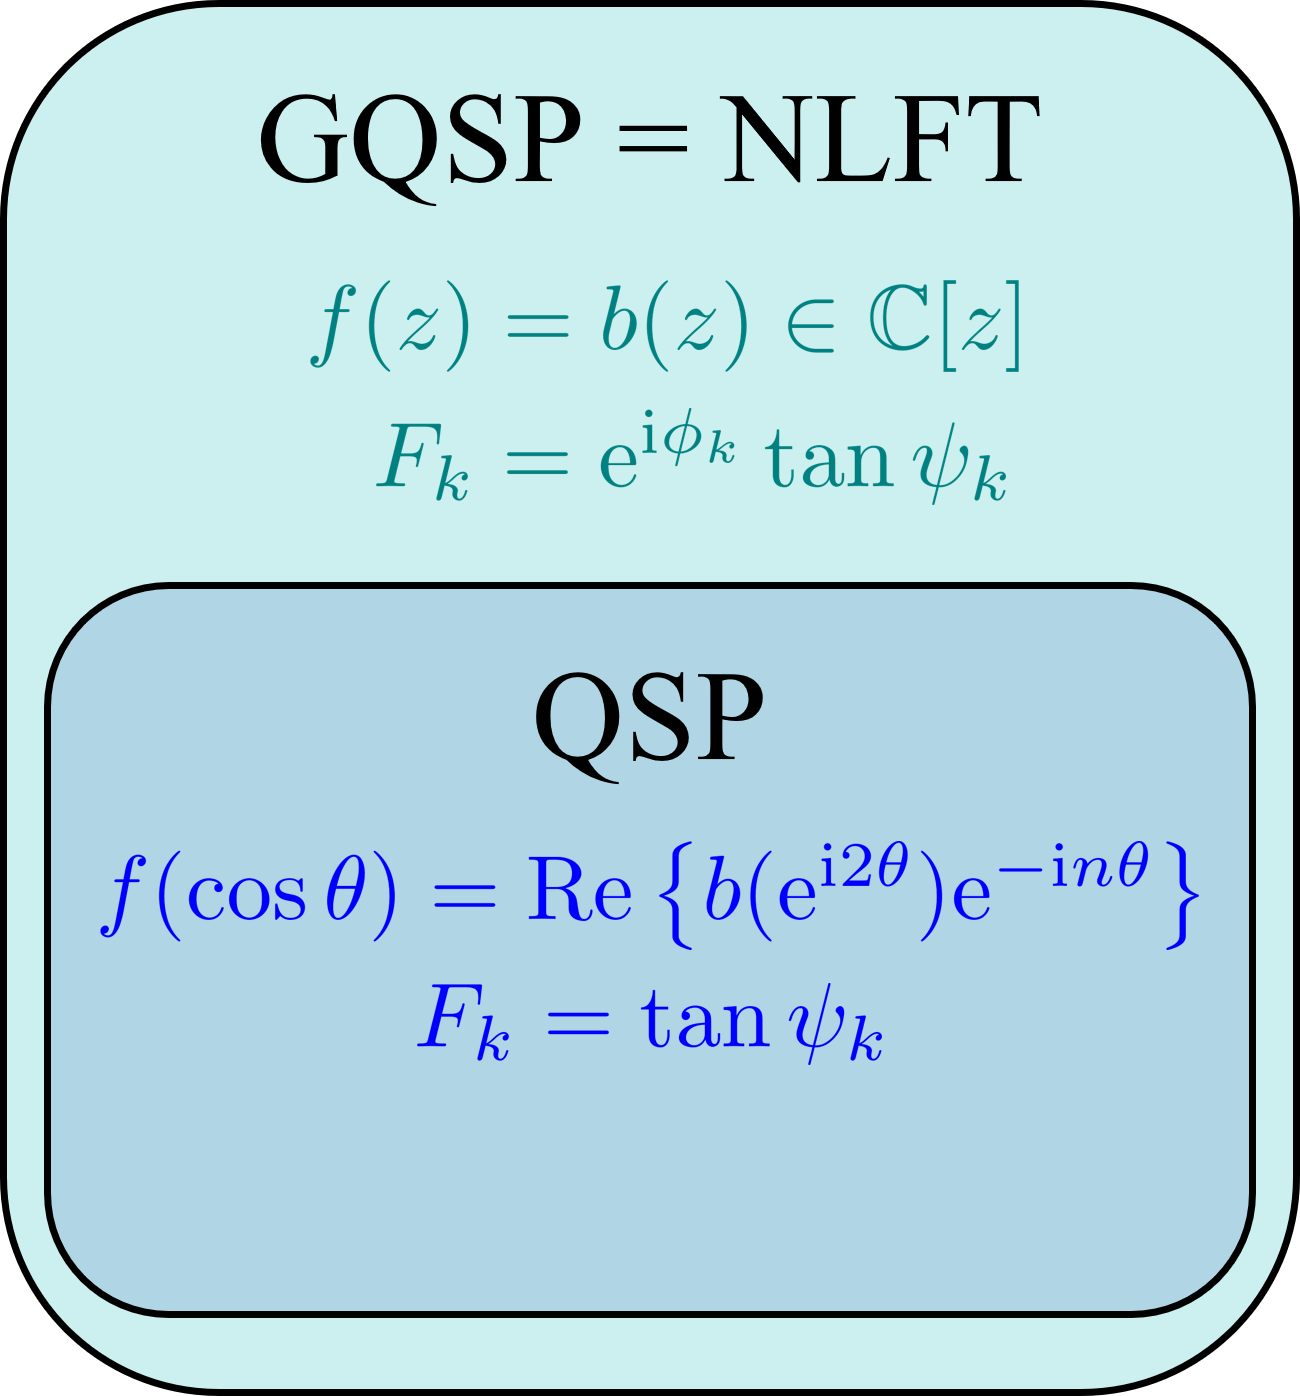
\includegraphics[width=1\linewidth]{figures/GQSP_NLFT_QSP.png}
            % \caption{Caption}
            % \label{fig:enter-label}
        \end{figure}
    \end{column}
    \end{columns}
\end{frame}
% \begin{frame}{QSP and NLFT}
%     Previously, for the symmetric phase $\Phi=(\psi_{\color{red}d},\ldots,\psi_{\color{red}1},\psi_0,\psi_1,\ldots,\psi_d)$, we have established that by setting $x=\cos\theta$, $z = \ee^{\ii2\theta}$, $F=(F_{\color{red}d},\ldots,F_{\color{red}1},F_0,F_1,\ldots,F_d)$ and $F_k=\ii\tan\psi_{\abs{k}}$,
%     \begin{align*}
%         V_\Psi(x) &= H \ee^{\ii d\theta Z} \mathcal{F}(z) \ee^{\ii d\theta Z} H \\
%         &= \left[\begin{matrix}
%             \frac{1}{2}\left(a(z)z^d + a^*(z)z^{-d} + b(z) - b^*(z)\right) & * \\ * & *
%         \end{matrix}\right].
%     \end{align*}
%     Hence, the target function is
%     \begin{equation}
%         f(x) = \mathrm{Im}\{P(x)\} = \mathrm{Im}\{b(z)\}
%     \end{equation}
%     with $z=\ee^{\ii2(\arccos x)}$.
% \end{frame}
\begin{frame}{NLFT}
    \begin{definition}[Nonlinear Fourier Transform]
        Let $F\in\ell^0(\mathbb{Z},\mathbb{C})$ be a compactly supported sequence on $[m:n]$, its $\mathrm{SU}(2)$ \textit{nonlinear Fourier transform} on $\mathbb{C}\cup\{\infty\}$ is defined as
        \begin{equation}
            \mathcal{F}(z) = (a,b) \defeq \overrightarrow{\prod_{k=m}^n} \frac{1}{\sqrt{1+\abs{F_k}^2}} \left[\begin{matrix}
                1 & F_kz^k \\ -\overline{F}_kz^{-k} & 1
            \end{matrix}\right].
        \end{equation}
    \end{definition}
    Sometimes, we often see $\mathcal{F}$ be denoted by
    \begin{equation*}
        \NLFT{F} \text{ or } \NLFT{[F_{m},\ldots,F_{n}]}.
    \end{equation*}
    But these are too space-consuming for this presentation, so we will not use them.
\end{frame}
\begin{frame}{GQSP and NLFT}
    GQSP and NLFT are connected by the following substitution:
    \begin{theorem}[GQSP $\equiv$ NLFT]
        Consider $f\in \mathbb{C}[z]$. By setting
        \begin{align}
            &b(z) = f(z) \\
            &F_k = \ee^{\ii\phi_k}\tan\psi_k\;\;\;(k\in[0:n]),
        \end{align}
        we have
        \begin{equation}
            \left[\begin{matrix}
                * & f(z) \\ * & *
            \end{matrix}\right] = \left[\begin{matrix}
                a(z) & b(z) \\ -b^*(z) & a^*(z)
            \end{matrix}\right] \left[\begin{matrix}
                z^n \\ & 1
            \end{matrix}\right].
        \end{equation}
    \end{theorem}
\end{frame}

\begin{frame}{Tasks}
    \textbf{Task (QSP)}:\\
    Given an even or odd polynomial $f(x)\in\mathbb{R}[x]$ of degree $n$ satisfying $\norm{f}_\infty\le1$, find a sequence $\Psi$ such that $f(x) = \mathrm{Im}\{\langle0|V_\Psi(x)|0\rangle\}$. 
    $$\downarrow$$
    \textbf{Task (inverse NLFT)}:\\
    Given a Laurent polynomial $b(z)$, determine a complementary Laurent polynomial $a(z)$ and a compactly supported sequence of Fourier coefficients $F$ such that $\mathcal{F} = (a,b)$.
\end{frame}

%%%%%%%%%%%%%%%%%%%%%%%%%%%%%%%%%%%%%%%%%%%%%%%%%%%%%%%%%%%%%%%%%%%%%%%
\subsection{Properties}
\begin{frame}{Properties of NLFT -- Shifting Property}
    \begin{theorem}[Laurent Polynomials]
        If the sequence $F = (\ldots,0,F_{m},F_{m+1},\ldots,F_{n})$, then for $\mathcal{F}=(a(z),b(z))$,
        \begin{align*}
            &a(z) = a_{m-n} z^{m-n} + \cdots + a_0 &b(z) = b_mz^m + \cdots + b_nz^n.
        \end{align*}
    \end{theorem}
    
    % \begin{proof}
    %     The proof is by induction and is trivial.
    % \end{proof}
    % \vspace{1em}
    % \hrule
    % It can be seen that $a(z) \in \mathcal{H}^2(\mathbb{D}^*)$. As for the case where $F$ is symmetric, and $b(z) = \ii f(x)$ for $f$ an even polynomial of degree $2d$,
    % \begin{align*}
    %     f(x) &= \sum_{k=0}^{d} t_k T_{2k}(x) = t_0 + \sum_{k=1}^{d} \frac{t_k}{2} \left(\ee^{\ii2k\theta} + \ee^{-\ii2k\theta}\right) = t_0 + \sum_{k=1}^d \frac{t_k}{2}(z^k + z^{-k}) = -\ii b(z).
    % \end{align*}

    \begin{theorem}[Shifting Property]
        Consider the sequence $\{F_k\}$ having the NLFT $\mathcal{F} = (a(z),b(z))$. Then for the sequence $\{G_k\}$ satisfying $G_k = F_{k-1}$,
        \begin{equation}
            \mathcal{G} = \left(a(z),z b(z)\right).
        \end{equation}
    \end{theorem}

    From the above two results, we can set $F$ to be \textit{supported} on $[0:n]$ without loss of generality. Henceforth, both $a^*$ and $b$ are degree $n$ polynomials in $z$.
\end{frame}

\begin{frame}{Properties of NLFT}
    Consider $\mathcal{F} = (a(z),b(z))$. Since for $z$ on $\mathbb{T}$, $\mathcal{F}\in\mathrm{SU}(2)$, we have
    \begin{equation*}
        \abs{a(z)}^2 + \abs{b(z)}^2 = 1.
    \end{equation*}
    Thus, for all $z\in \mathbb{C}\cup\{\infty\}$,
    \begin{equation}
        {\color{red} a(z) a^*(z) + b(z) b^*(z) = 1}.
    \end{equation}
    \hrule
    A simple example will be $F = (F_0,F_1,F_2) = (0,1,1)$:
    \begin{align*}
        \mathcal{F} &= \frac{1}{2}\left[\begin{matrix}
            1 & z \\ -z^{-1} & 1
        \end{matrix}\right] \left[\begin{matrix}
            1 & z^2 \\ -z^{-2} & 1
        \end{matrix}\right] = \frac{1}{2} \left[\begin{matrix}
            1 - z^{-1} &  z + z^2 \\ -(z^{-1}+z^{-2}) & 1-z
        \end{matrix}\right], \\
        \Rightarrow\, & aa^* + bb^* = \frac{1}{4}\left((-z+1+1-z^{-1}) + (z+1+1+z^{-1})\right) = 1.\;\;\;\;\; \square
    \end{align*}
\end{frame}
\begin{frame}{Properties of NLFT}
    We note that
    \begin{align*}
        a^*(0) = \prod_{k=0}^{n} \frac{1}{\sqrt{1+\abs{F_k}^2}} > 0.
    \end{align*}
    Thus we introduce the following lemma (Lemma 2.2 in \cite{Lin2025}):
    \begin{lemma}[NLFT Bijection]
        The NLFT is a bijection from $\ell_0(\mathbb{Z},\mathbb{C})$ onto the space
        \begin{equation}
            \mathbf{S} \defeq \setdef{(a,b)}{a,b\text{ are Laurent polynomials, }aa^*+bb^*=1\text{, }0<a^*(0)<\infty}.
        \end{equation}
    \end{lemma}
    The polynomials $a$ and $b$ are \textit{complementary} to each other. As a corollary, if a valid $b$ is given, then there exists a {\color{red}unique outer} $a^*$ such that $(a,b)\in\mathbf{S}$. Constructing the polynomial $a^*$ requires the \textit{\color{blue}Weiss algorithm}.
\end{frame}
\begin{frame}{Outer Functions}
    \begin{definition}[Outer Function]
        An outer function is a function that has no zeros in $\mathbb{D}$.
    \end{definition}

    \begin{lemma}[Outer Function]
        A function $g\in L^\infty(\mathbb{T})$ is outer if 
        \begin{equation}
            \log\abs{g}\in L^1(\mathbb{T}) \text{, } g=\ee^G \text{, and } G=\log\abs{g} + \ii \mathcal{H}(\log\abs{g}).
        \end{equation}
        The function $\mathcal{H}$ is the Hilbert transform:
        \begin{equation}
            \mathcal{H}(c) = 0 \text{, } \mathcal{H}(z^n) = -\ii z^n \text{, } \mathcal{H}(z^{-n}) = \ii z^{-n}.
        \end{equation}
    \end{lemma}
\end{frame}
% \begin{frame}{Outer Functions}
%     proof
    
%     Inner-Outer factorization
% \end{frame}
\begin{frame}{Properties of NLFT -- Szeg\H{o} Condition}
    Given a function $b$, can we find another function $a$ such that $(a,b)$ is the NLFT of a sequence?

    The answer is positive! See theorem 4 in \cite{Szego}:
    \begin{lemma}[Szeg\H{o} Condition]
        Consider a measurable function $b$ on $\mathbb{T}$ with $\norm{b}_\infty<1$. If $b$ satisfies the Szeg\H{o} condition
        \begin{equation}
            \int_{\mathbb{T}} \log(1-\abs{b}^2)\,\dd z > -\infty,
        \end{equation}
        then there exists a \textit{unique} measurable outer function $a^*$ on $\mathbb{T}$ such that $(a,b)\in\mathbf{S}$.
    \end{lemma}
    
    This condition is natural: $\abs{a(z)}^2 = 1-\abs{b(z)}^2$ is $>0$ almost everywhere on $\mathbb{T}$.
\end{frame}

% \begin{frame}{Properties of NLFT}
%     In literature, one often see a decreasing family of subsets
%     \begin{equation}
%         \mathbf{S}_\eta \defeq \setdef{(a,b)\in\mathbf{S}}{b\text{ is a polynomial, }0<\sup_{z\in\mathbb{T}}\abs{b(z)}\le1-\eta}.
%     \end{equation}
%     As $\eta\in(0,1)$ approaches one, the inverse NLFT problem is ill-conditioned, and it becomes harder to find the phase sequence.

%     Furthermore, for $(a,b)\in\mathbf{S}$ and $a^*$ is outer, if $(a,b)\in\mathbf{S}_\eta$, then $a^*$ has no zeros on $\overline{\mathbb{D}}$.
% \end{frame}

%%%%%%%%%%%%%%%%%%%%%%%%%%%%%%%%%%%%%%%%%%%%%%%%
% \begin{frame}{Properties of NLFT -- Shifting}
    
%     \begin{proof}
%         The proof is by induction:
%         \begin{align*}
%             \left[\begin{matrix}
%                 a_{k-1} & zb_{k-1} \\ * & *
%             \end{matrix}\right] \left[\begin{matrix}
%                 1 & F_kz^{k+1} \\
%                 * & *
%             \end{matrix}\right]  &= \left[\begin{matrix}
%                 a_{k-1} - F_k^*z^{-k} b_{k-1} & a_{k-1}F_kz^{k+1} + zb_{n-1} \\ * & *
%             \end{matrix}\right] \\
%             &= \left[\begin{matrix}
%                 a_k(z) & zb_k(z) \\ * & *
%             \end{matrix}\right]
%         \end{align*}
%         Thus it is shown.
%     \end{proof}
% \end{frame}

% \begin{frame}{Properties of NLFT}
%     Since we can easily obtain the NLFT of a shifted sequence, without loss of generality, let us consider sequences starting always from 0, i.e.
%     \begin{equation}
%         F = [F_0,F_1,\cdots,F_n].
%     \end{equation}
%     Then, for $\mathcal{F}=(a,b)$, both $a^*$ and $b$ are degree $n$ polynomials in $z$.
% \end{frame}

%%%%%%%%%%%%%%%%%%%%%%%%%%%%%

\begin{frame}{Properties of NLFT -- Riemann--Hilbert Factorization}
    We can decompose $F$ into the two disjoint sequences $F_{<k}=(F_{0},\ldots,F_{k-1},0,\ldots)$ and $F_{\ge k}=(0,\ldots,0,F_k,\ldots,F_{n})$. Then, the corresponding NLFT will have the factorization
    \begin{equation}
        \underbrace{\left[\begin{matrix}
            a(z) & b(z) \\ -b^*(z) & a^*(z)
        \end{matrix}\right]}_{\mathcal{F}} = \underbrace{\left[\begin{matrix}
            a_{<k}(z) & b_{<k}(z) \\ -b_{<k}^*(z) & a_{<k}^*(z)
        \end{matrix}\right]}_{\mathcal{F}_{<k}} \underbrace{\left[\begin{matrix}
            a_{\ge k}(z) & b_{\ge k}(z) \\ -b_{\ge k}^*(z) & a_{\ge k}^*(z)
        \end{matrix}\right]}_{\mathcal{F}_{\ge k}}.
    \end{equation}

    This is the {\color{blue}Riemann--Hilbert factorization} of $\mathcal{F}$.
    The resulting polynomials are parameterized by
    \begin{align}
        a_{\ge k}^*(z) &= a_{k,0} + a_{k,1}z + \cdots + a_{k,n-k}z^{n-k},\\
        b_{\ge k}(z) &= z^k \left(b_{k,0} + b_{k,1}z + \cdots + b_{k,n-k}z^{n-k}\right).
    \end{align}
\end{frame}

\begin{frame}{Properties of NLFT -- Layer-Stripping}
    Consider the sequence $F = (F_0,F_1,F_2,\ldots)$ factorized into $F_{<1}$ and $F_{\ge1}$. Then
    \begin{align*}
        \mathcal{F}_{\ge1} = \left[\begin{matrix}
            a_{\ge1}(z) & b_{\ge1}(z) \\ -b_{\ge1}^*(z) & a_{\ge1}^*(z)
        \end{matrix}\right] = \frac{1}{\sqrt{1+\abs{F_0}^2}}\left[\begin{matrix}
            1 & -F_0 \\ \overline{F}_0 & 1
        \end{matrix}\right] \cdot \left[\begin{matrix}
            a(z) & b(z) \\
            -b^*(z) & a^*(z)
        \end{matrix}\right],
    \end{align*}
    with $d(z)$ a polynomial having smallest power 1. Henceforth,
    \begin{align*}
        b_{\ge1}(z) &\propto b(z) - F_0 a^*(z) \\
        0 = b_{\ge1}(0) &= b(0) - F_0 a^*(0) \\
        \Rightarrow F_0 &= \frac{b(0)}{a^*(0)} = \frac{b_{\ge0}(0)}{a_{\ge0}^*(0)} = \frac{b_{0,0}}{a_{0,0}}.
    \end{align*}
\end{frame}
\begin{frame}{Properties of NLFT -- Layer-Stripping}
    \begin{theorem}[Layer-Stripping]
        Consider $\mathcal{F}=(a,b)$ as the NLFT of $F = (F_0,F_1,\ldots,F_n)$ with RH factorization $\mathcal{F}=\mathcal{F}_{<k}\mathcal{F}_{\ge k}$, then
        \begin{equation}
            F_k =  \left.\frac{b_{\ge k}(z) z^{-k}}{a_{\ge k}^*(z)}\right|_{z=0} = \frac{b_{k,0}}{a_{k,0}}.
        \end{equation}
    \end{theorem}
    \begin{proof}
        Proof by combining the shifting property, $F_0 = b_{\ge0}(0) / a_{\ge0}^*(0)$, and the parameterization of the polynomials $a_{\ge k}^*$ and $b_{\ge k}$.
    \end{proof}

    The layer-stripping method in NLFT is EXACTLY the SAME as the layer-stripping method developed in \cite{Tsai,GSLW18}.
\end{frame}


\begin{frame}{Properties of NLFT -- Riemann--Hilbert Factorization}
    \begin{theorem}[Riemann--Hilbert Factorization]
        Let $P_{\mathbb{D}}$ be the projection of a Laurent polynomial onto its non-negative powers, and $P_{\mathbb{D}^*}$ the projection onto the non-positive powers:
        \begin{equation}
            \left[\begin{matrix}
                1 & P_{\mathbb{D}^*}\frac{b^*}{a^*} \\
                -z^k P_{\mathbbm{D}}z^{-k}\frac{b}{a} & 1
            \end{matrix}\right] \left[\begin{matrix}
                a_{\ge k} \\ b_{\ge k}
            \end{matrix}\right] \propto \left[\begin{matrix}
                1 \\ 0
            \end{matrix}\right].
        \end{equation}
    \end{theorem}
    \begin{proof}
    By observing the order to the polynomials, we have
    \begin{center}
        \resizebox{0.7\linewidth}{!}{$
            \begin{aligned}
                &\left(a_{<k},b_{<k}\right) = \left(a,b\right) \left(a_{\ge k}^*,-b_{\ge k}\right) = \left(aa_{\ge k}^* + bb_{\ge k}^*, -ab_{\ge k} + a_{\ge k}b\right) \\
                &\Rightarrow \begin{cases}
                    b_{\ge k} = \frac{ba_{\ge k}}{a} - \frac{b_{<k}}{a} \Rightarrow b_{\ge k} = z^k P_{\mathbb{D}}\left(z^{-k}\frac{b}{a}\right) a_{\ge k} \\
                    a^*_{\ge k} = \frac{1}{a_{\ge k}(0)} - P_{\mathbb{D}}\left(\frac{b}{a}\right) b^*_{\ge k}
                \end{cases}.
            \end{aligned}$
        }
    \end{center}
    Thus it is shown, with the proportionality constant being $a_{\ge k}^*(0)$.
    \end{proof}
\end{frame}


% % \begin{frame}{Properties of NLFT -- Szeg\H{o} Condition}
% %     How do we construct $a(z)$ from $b(z)$? Some inspirations:
% %     \begin{itemize}
% %         \item $\abs{a(z)} = \sqrt{1-\abs{b(z)}^2}$,
% %         \item $a(z)$ only has non-positive powers of $z$.
% %         \item $a(z)>0$ a.e. on $\mathbb{T}$.
% %     \end{itemize}
% %     Then
% %     \begin{align*}
% %         a(z) &= \exp\left(G(z)\right) &(G\sim \log\sqrt{1-\abs{b}^2}).
% %     \end{align*}
% %     If $R(z) = \log\sqrt{1-\abs{b}^2} = \cdots + r_{-1}z^{-1} + r_0 + r_1z + \cdots$, let $G(z) = \cdots + r_{-1}z^{-1} + 2r_0$, then
% %     \begin{equation}
% %         a(z) = \exp(G(z)) = \exp(\cdots + r_{-1}z^{-1} + 2r_0).
% %     \end{equation}
    
    
% % \end{frame}

% \begin{frame}{Set of Functions}
%     Let us formally define some special sets
%     \begin{definition}[Functions of NLFT]
%         Define the set of all possible NLFT of a sequence $F$ on $\mathbb{Z}$ as
%         \begin{equation}
%             \mathbf{B} \defeq \setdef{(a,b)}{aa^*+bb^*=1 \text{ a.e. on }\mathbb{T}, a\in\mathcal{H}(\mathbb{D}^*), a(\infty)>0,...}.
%         \end{equation}
%     \end{definition}
%     % \color{red}Szeg\H{o} condition and create $a(z)$ from $b(z)$.
    
%     % $(a,b)\in B,L,H...$
% \end{frame}